\section{Course Management}
Another important sector in which AllSpark is involved is provide formation
courses and certifications for IT professionals. The teacher personal for
these courses are selected and trained among the developers and sysadmins
who works for AllSpark. 

The importance of this sector is underlined by the growing need for this
kind of certifications in many fields of information technologies related
applications.

The aim of AllSpark is to provide a service to many professionals who need
to certificate their knowledge and experience in various fields. On the
other hand this is a possibility to gain renown as a reliable authority for
delivering these services.

Organizing this section particular attention has been posed in defining
compatible timetables among the different courses, and assure the
up-to-date state of the study material and case studies presented.

The selection of the lecturers is also a vital task in order to organize a
successful course. AllSpark gives major importance to the experience of
their workers and to their ability in giving lectures, when selects the
lecturer for a course.

\subsection{Timetable management}
This process, represented in figure \ref{2img:timetable}  describes the
procedure needed in order to provide a consistent and non overlapping
schedule of the course.

Is important to provide an allocation that respect the possible
dependencies among different courses and avoids overlapping among lectures
of different courses.

\begin{figure}[!ht]
\centering
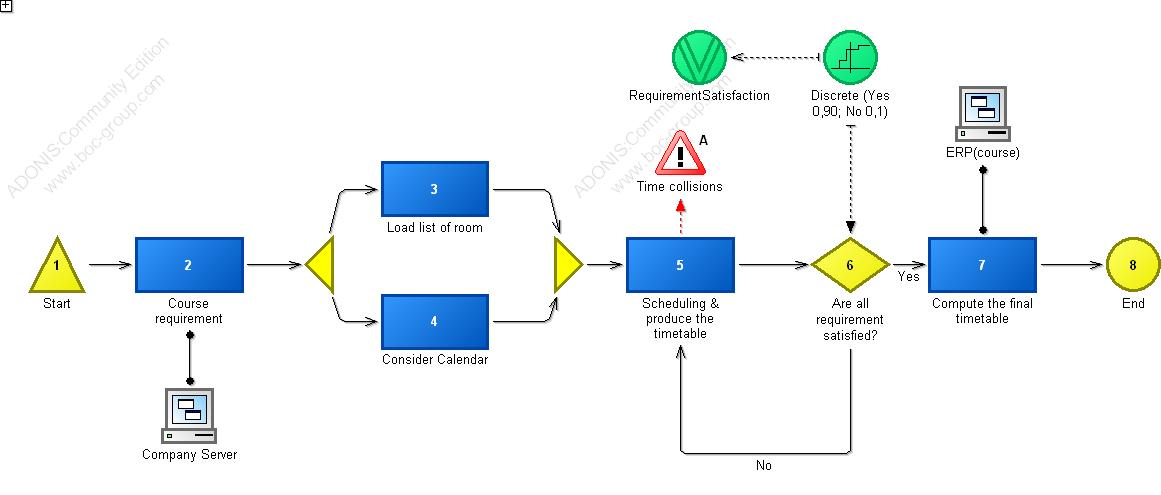
\includegraphics[scale=0.50,angle=90]{assign2/adonis/imgs/timetable.jpg}
\caption{Definition of the courses timetable}
\label{2img:timetable}
\end{figure}


\subsection{Course organization}
This process is one of the most important in this area, in fact it manages
the effective organization of a course. During this process the attention
is focused, on a firs phase on the teacher selection and the gathering of
course material and planning definition.

If needed the people selected for the teacher role can be trained on the
course methodologies. After this first phase, are preformed  some
activities regarding the definition of the courses structure, the presence
of practical lessons, possible correlation with other courses and the
examination details.

All these informations are then integrated and published. The structure of
this process can be seen in figure \ref{2img:course_organization}.

\begin{figure}[!ht]
\centering
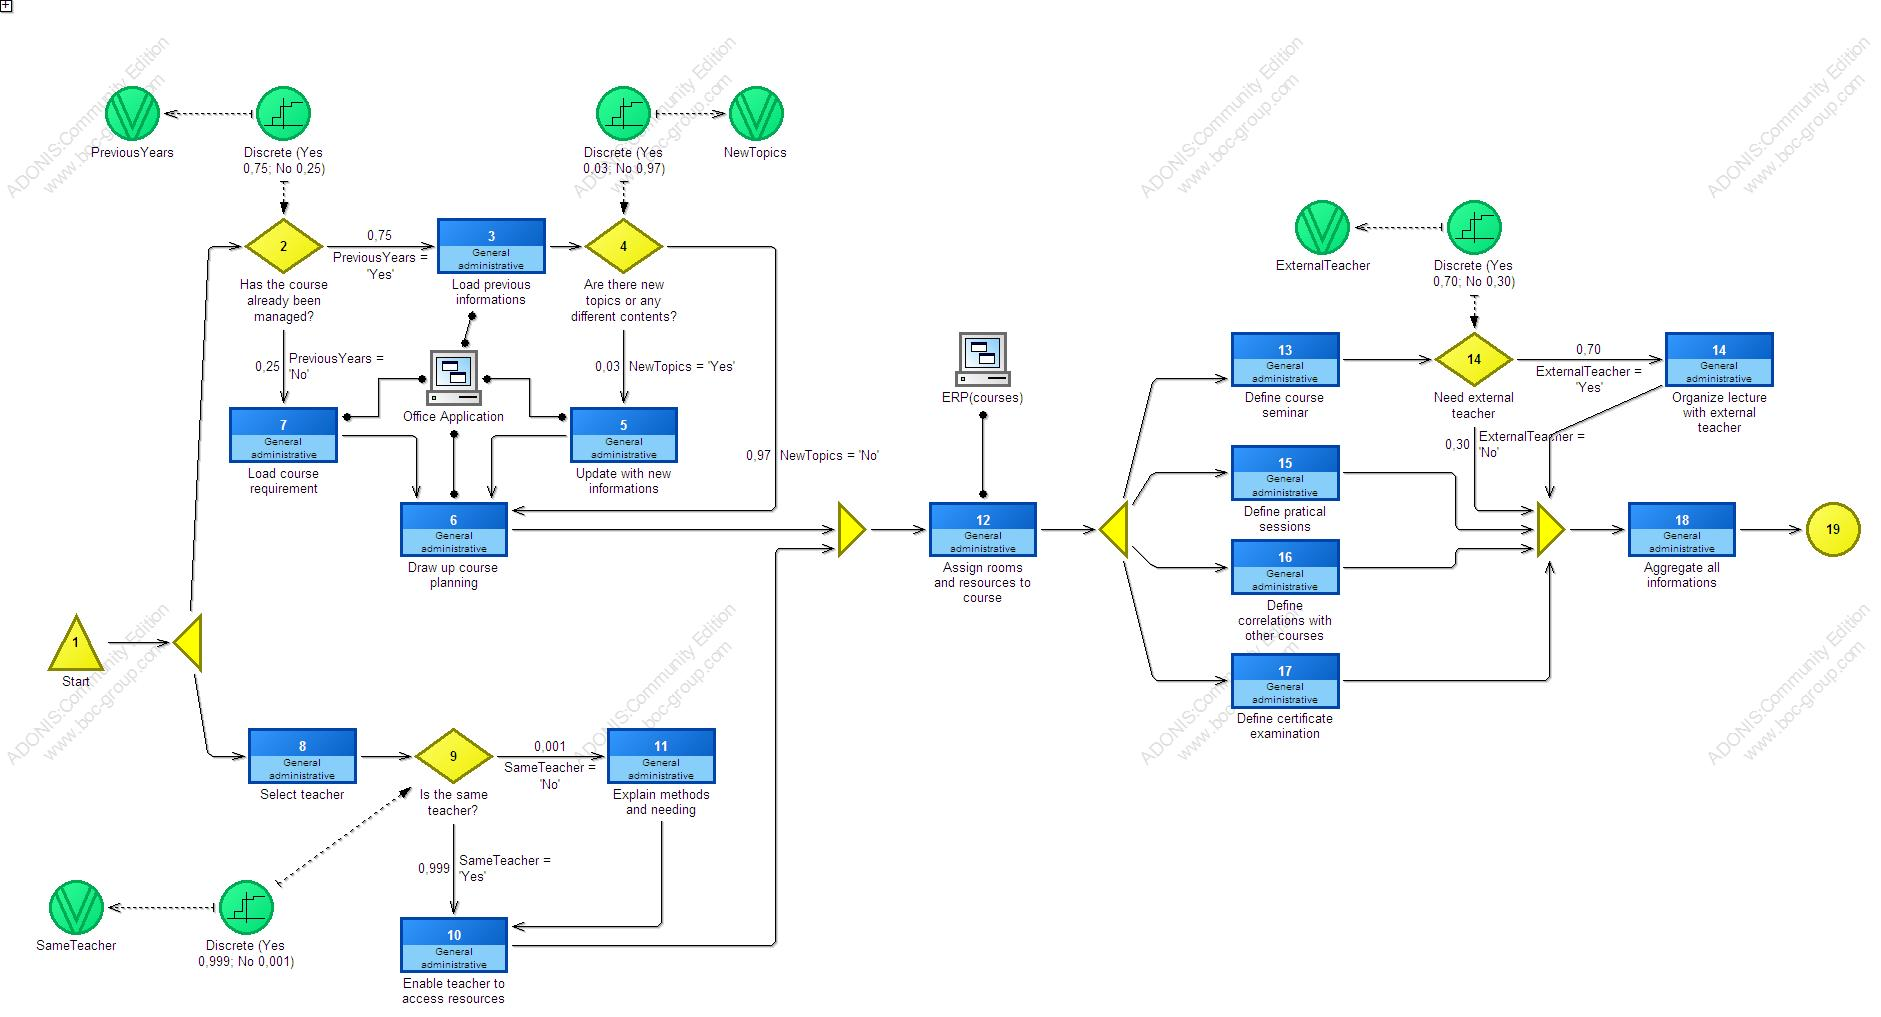
\includegraphics[scale=0.27, angle=90]{assign2/adonis/imgs/course_organization.jpg}
\caption{Organization of a formative course}
\label{2img:course_organization}
\end{figure}

\subsection{Course Material Management}
This process, as in figure \ref{2img:course_material}, represents the way
in which AllSpark manages the material needed as support for a course.
Obviously in order to provide a right choice of material is necessary to
analyze deeply the course scope.

Other important things are the quality of the material offered and its
consistency, in terms of completeness and correctness. AllSpark uses its
own infrastructure in order to offer a sort of reliable repository of
course material and documentation. The access to this repository is
scheduled consistently with the course schedule.

\begin{figure}[!ht]
\centering
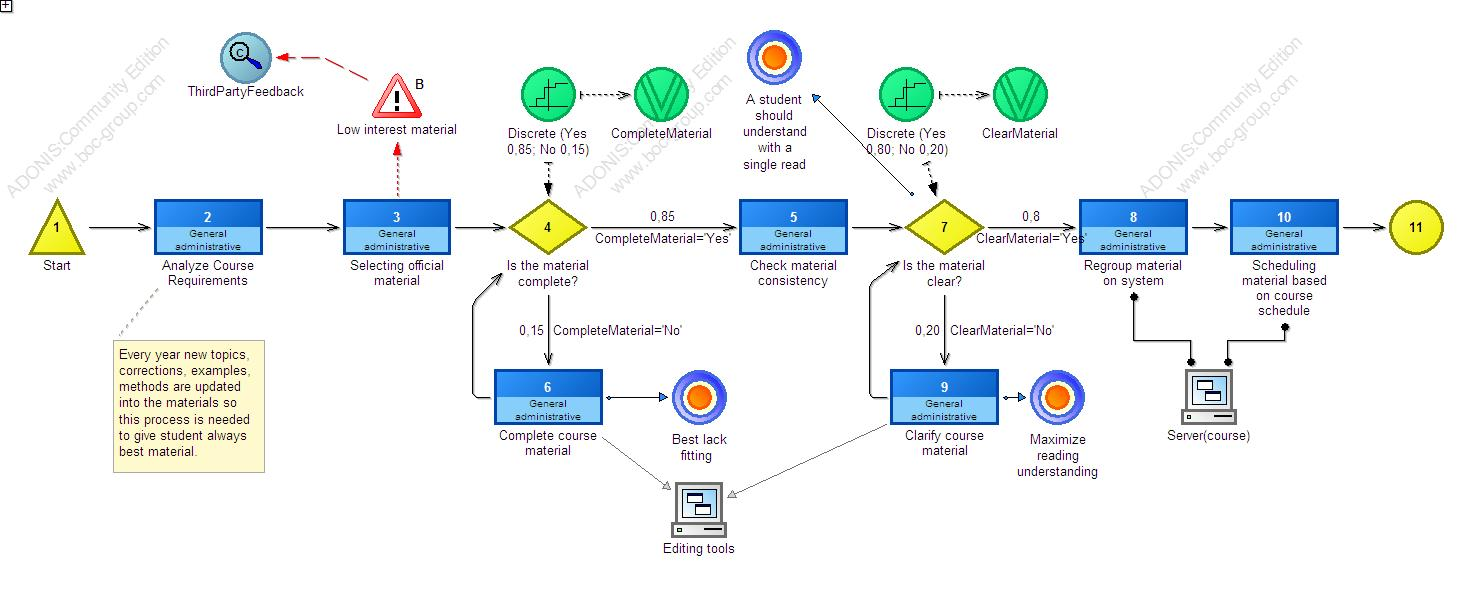
\includegraphics[scale=0.45, angle=90]{assign2/adonis/imgs/course_material.jpg}
\caption{Gathering and evaluation of course material}
\label{2img:course_material}
\end{figure}

\subsection{Examinations}
At the end of the most of the courses, an official examination is planned,
this is very important in order to achieve the goal of gain renown as a
certification authority. In fact the AllSpark standard in this area is to
keep the level of the course and of the examination quite high, in order to
add an ulterior value to our certifications.

Often AllSpark provides examination service for other Authorities, in this
case is necessary to retrieve from them the original text and organize the
examination over that particular test.

Difficulties on this process can be originated by the ambiguos nature of
some examination modalities, like for example open questions, which can
lead to misjudgement and wrong results in the evaluation.
The process is described by figure \ref{2img:examination}.

\begin{figure}[!ht]
\centering
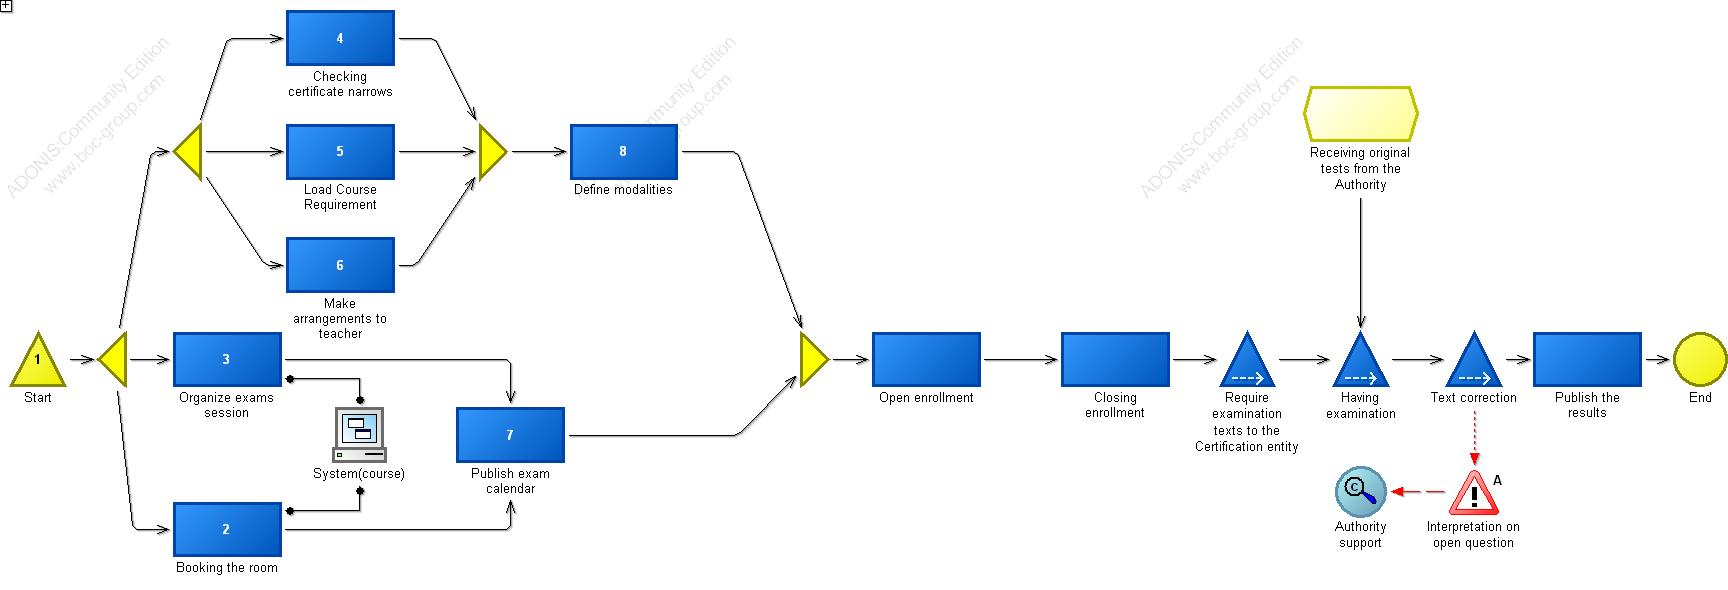
\includegraphics[scale=0.35, angle=90]{assign2/adonis/imgs/examination.jpg}
\caption{Organization of an examination test}
\label{2img:examination}
\end{figure}

\subsection{Certification management}
This process permits to manage the delivery of the certification to the
candidates who passed the examination. Often the certification is provided
by an external organization, for which AllSpark acts as an examination
authority. In this case in necessary to send them the list of approved
candidates, and retrieve the certification documents.

This process can handle the case in which a single certification is
considered as a hierarchy of other certifications, in this case all the
other documents are equally retrieved.

The image in figure \ref{2img:certification} describes this process. Here
the final document is customized with AllSpark logo and information.

\begin{figure}[!ht]
\centering
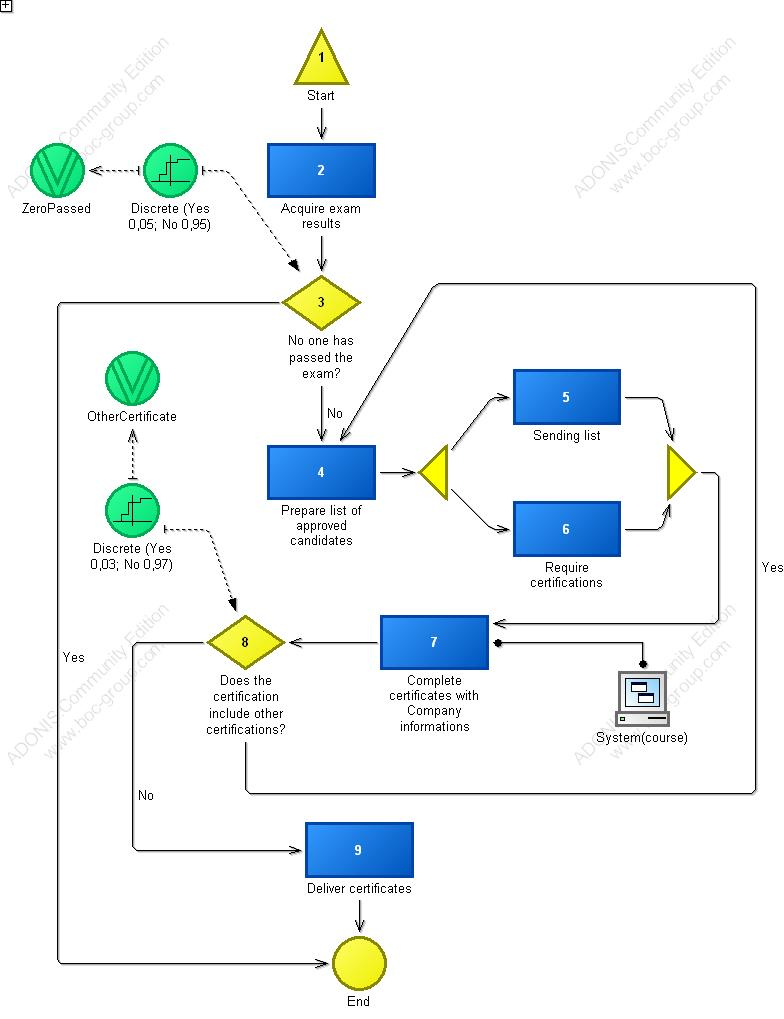
\includegraphics[scale=0.55]{assign2/adonis/imgs/certification.jpg}
\caption{Delivery of certification documents}
\label{2img:certification}
\end{figure}

